
\section {Evaluation}


In our evaluation, we demonstrate that:

\begin{itemize}
 \item The system can sustain very high throughput
 \item The system has extremely low latency for flow migrations
 \item The system is resilient to lossy network and update failure. 
\end{itemize}


The testbed we used for evaluation consists of two sets of machines: (i) four mid-range workstations (Quad-core Intel Xeon 3.7GHz, 32GB, 1Gbps NIC) and a conventional switch; and (ii) four high-end servers (16-core Intel Xeon 2.2GHz, 64GB, 40Gbps NIC) with an OpenFlow-enabled switch (we only use L-2 switching here). We conducted throughput stress tests in the four high-end servers, and unless specified, experiments are done in setting (i). 



\subsection{Throughput }

We show that an in-kernel implementation of the shim layer has very low overhead in the overall system. 


\begin{figure}[ht]
\centering
% 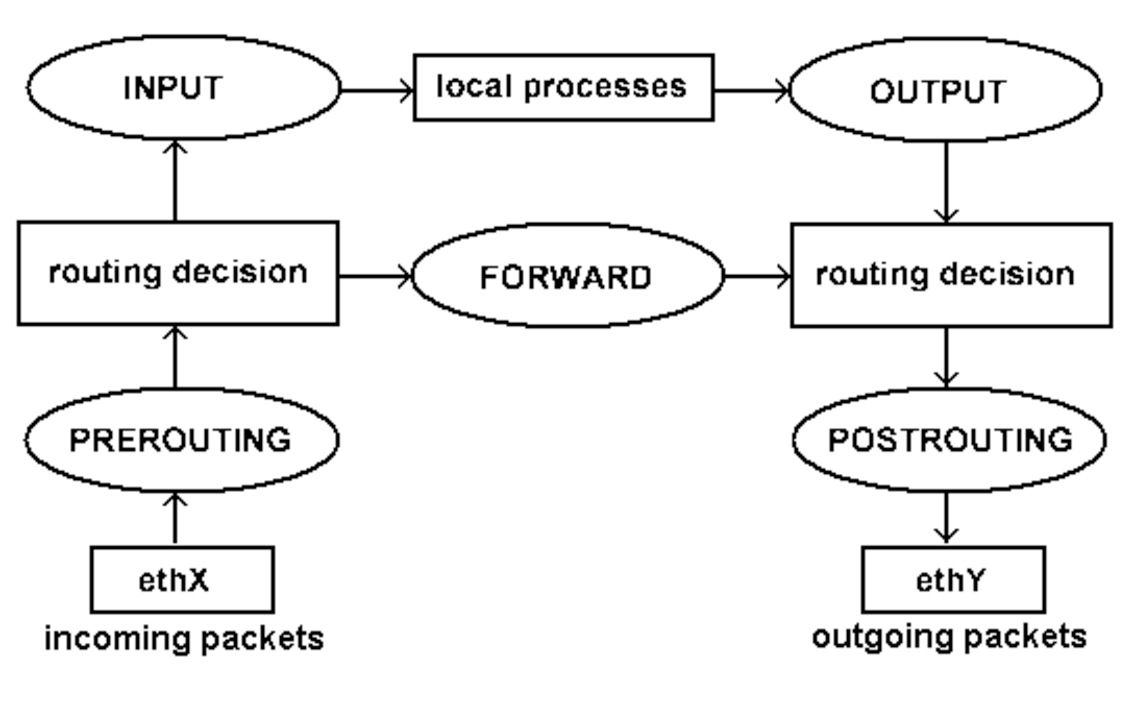
\includegraphics[scale=0.25]{figures/netfilter.pdf} 
% 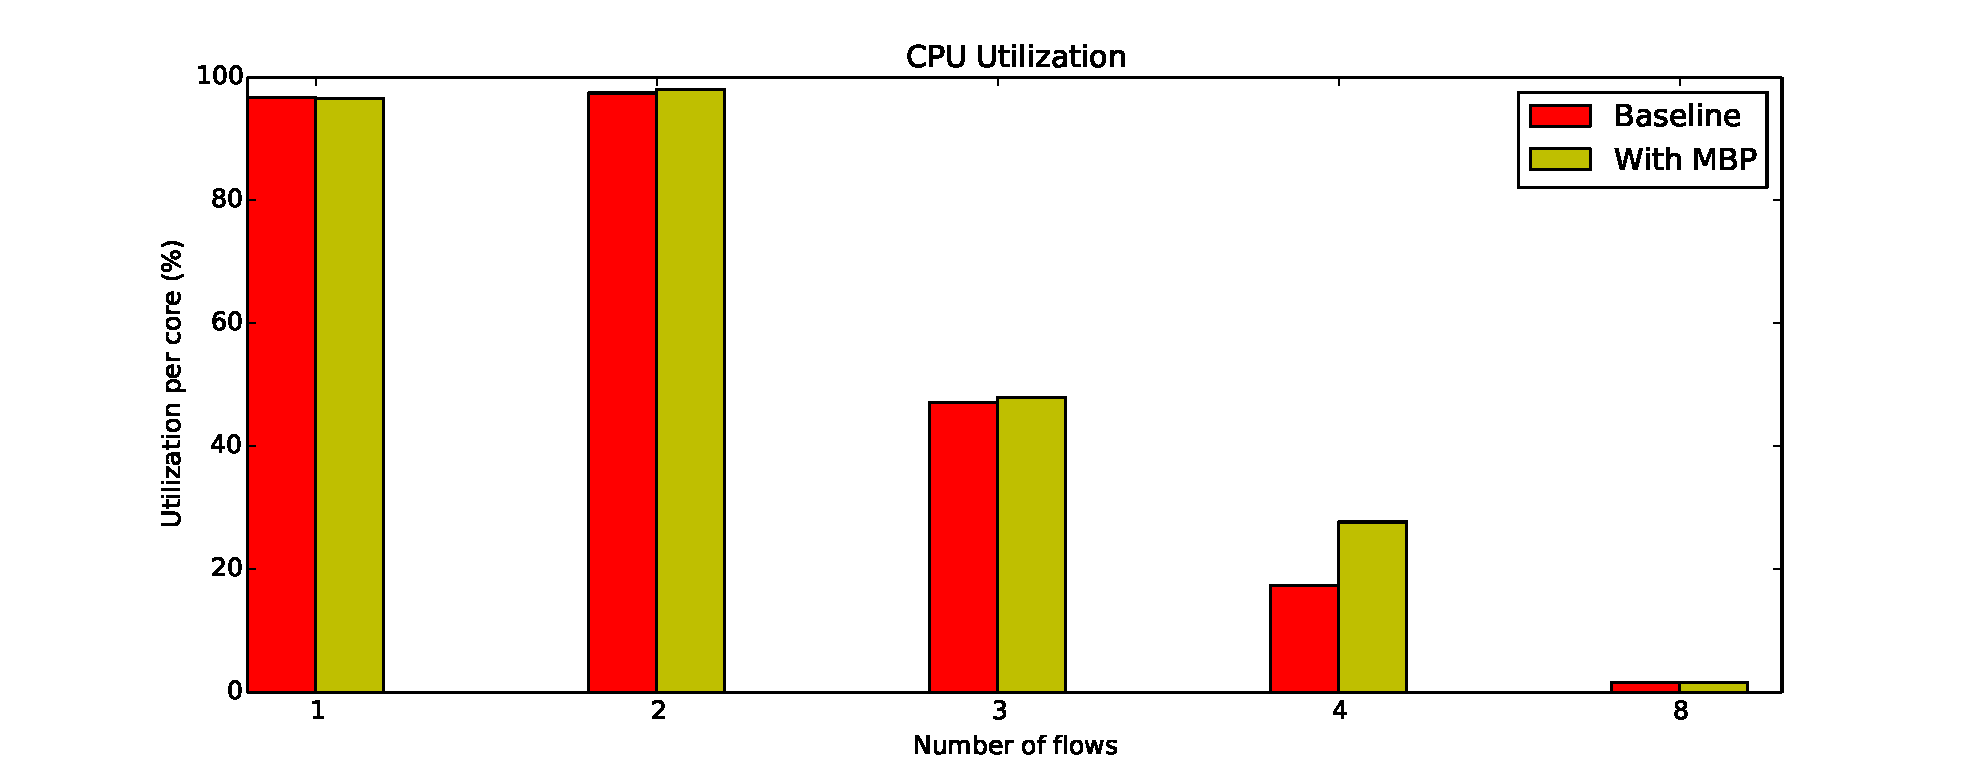
\includegraphics[width=0.53\linewidth]{figures/CPU.pdf} 
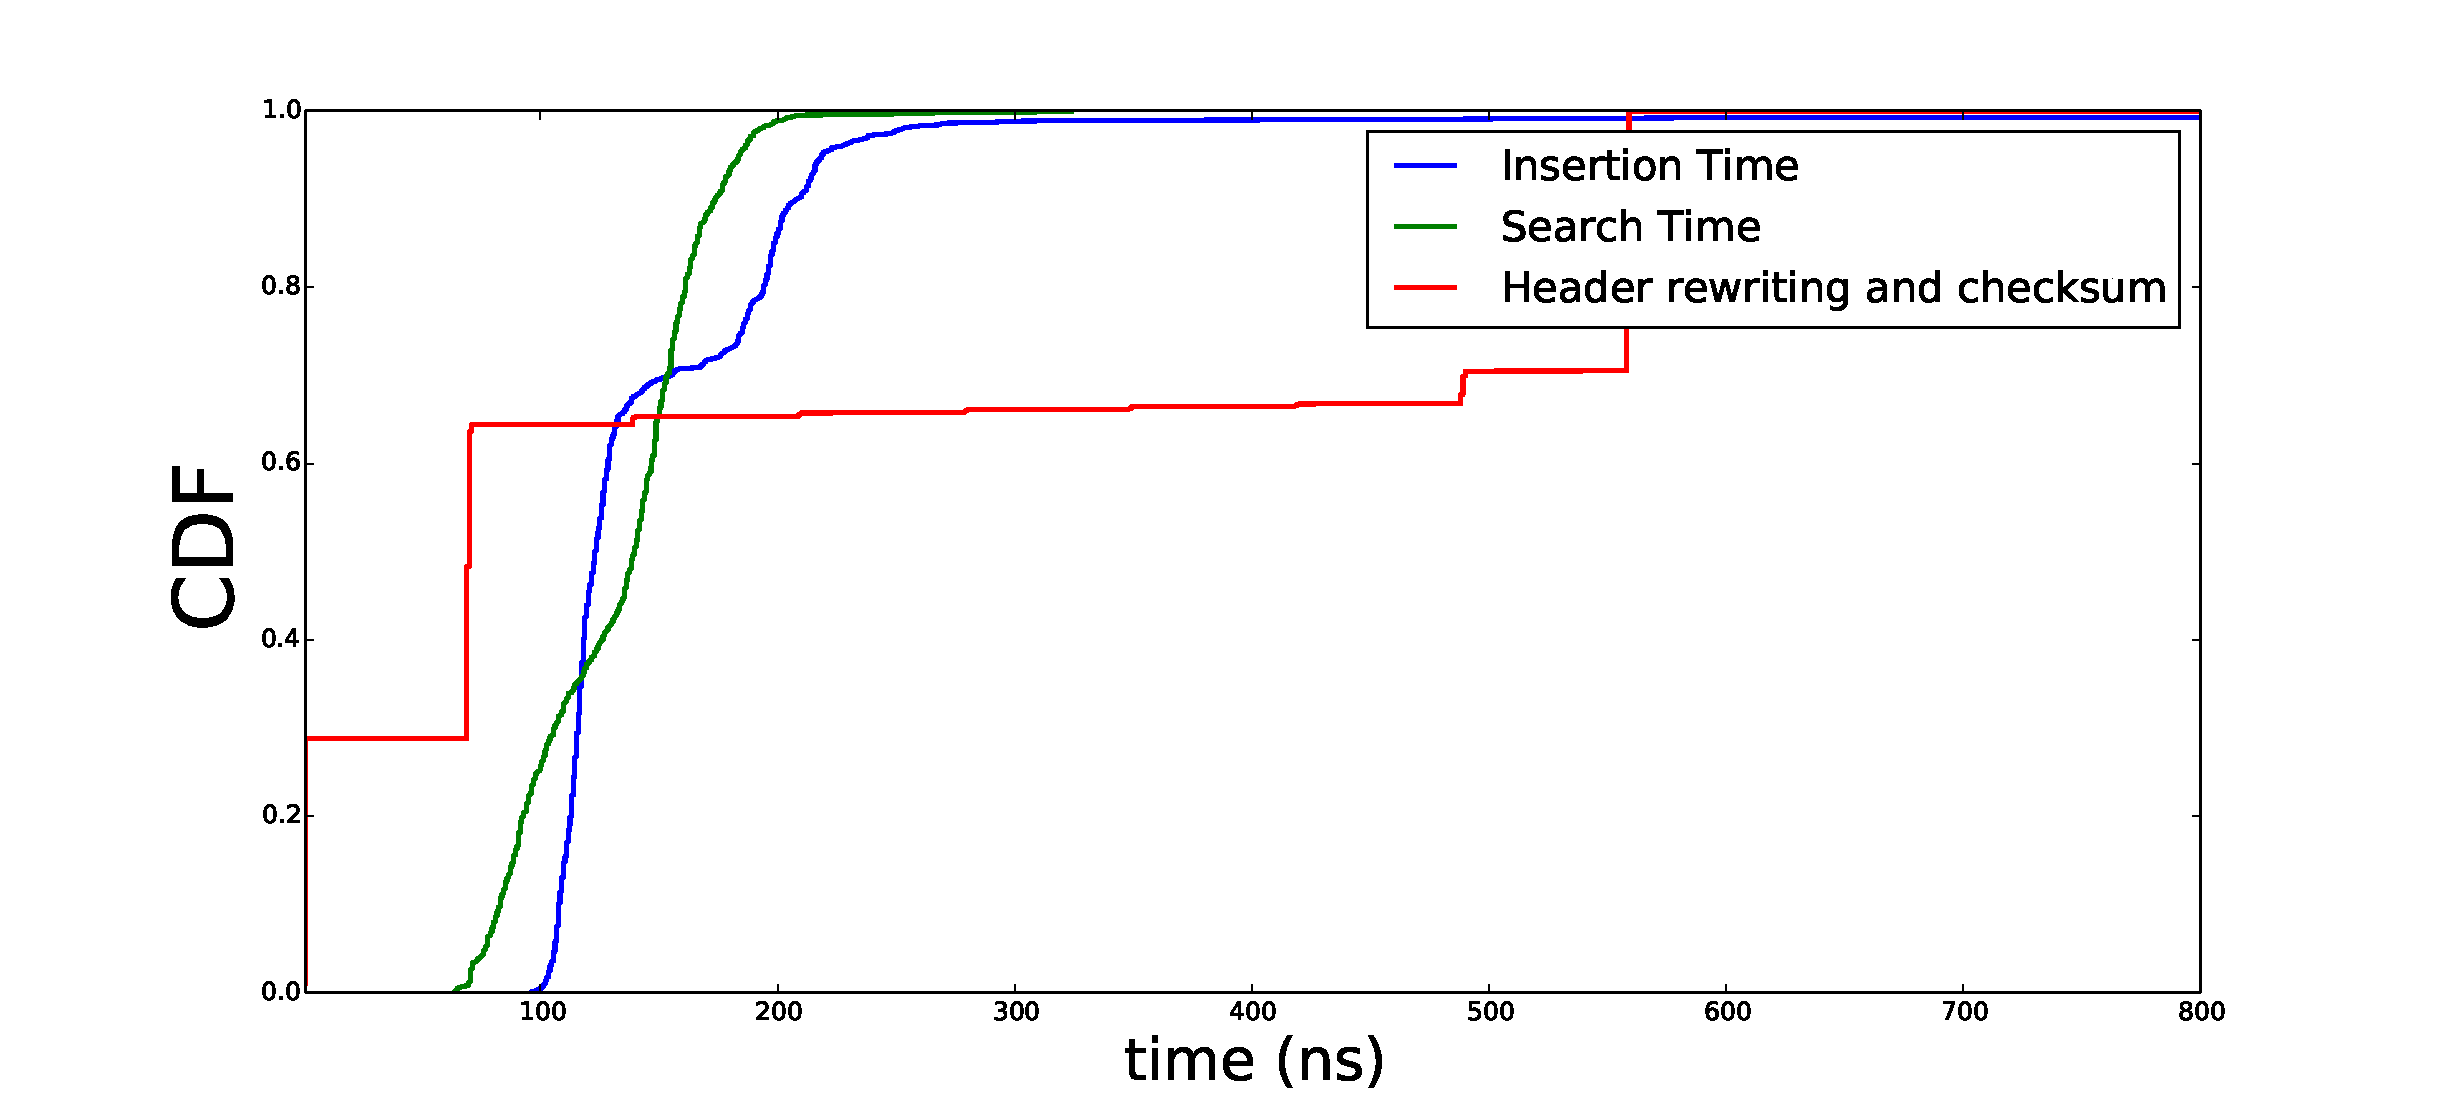
\includegraphics[width=\linewidth]{figures/cdf.pdf} 
\caption{\small Time CDF for different functions}\label{throughput}
\end{figure}
% 

The in-kernel implementation of the data plane includes three functions: (i) action hash lookup, (ii) header rewriting and re-checksum, (iii) rule installation. We also have a few optimizations in the data-plane implementation (e.g., partial checksum to reduce CPU cycle, a small hash table to fit in L3 cache) result in an extremely efficient system with a very low overhead.

We conducted a microbenchmark to see the delay different functions add to the system. We insert 100K rules in the kernel hash table, and conducted 100K lookup. We also microbenchmarked the header rewriting and partial checksum of the data packets. We had the two following methods to eliminate Linux timer's overhead: (i) batch and time the insertion and lookup for every one hundred rules; (ii) get the pure timer lookup time and then subtract that base number. The result shows that lookup, insertion and header rewriting takes on average 131, 251, and 214 ns, this gives us $\approx $ 2.8M packets per seconds with lookup and header rewriting, this is equivalent to 33.6 Gbps per core with MTU of 1500 Bytes.



\begin{figure}[ht]

\centering
% 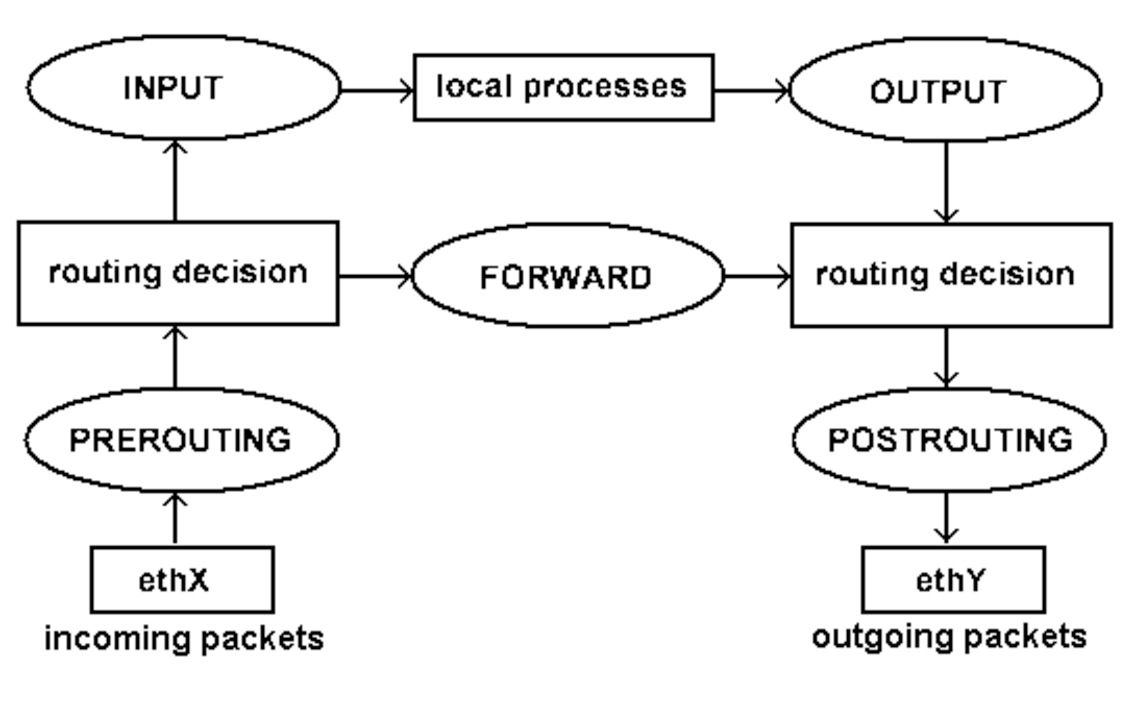
\includegraphics[scale=0.25]{figures/netfilter.pdf} 
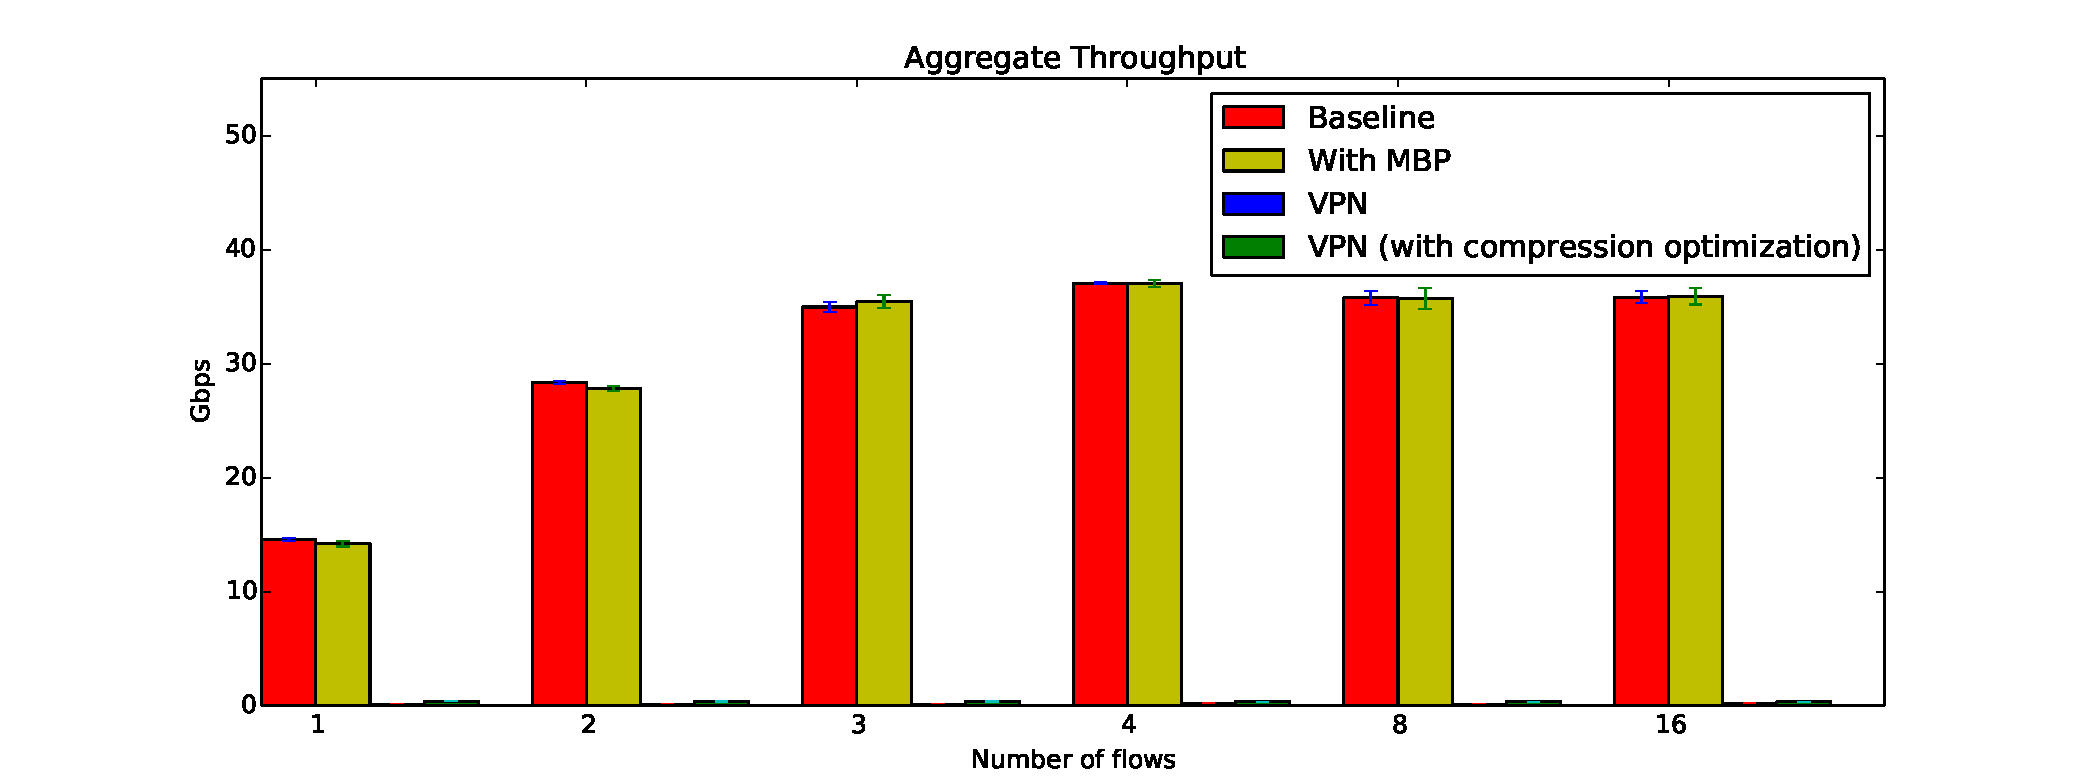
\includegraphics[width=\linewidth]{figures/throughput.pdf} 

\caption{\small Throughput of different approaches. The throughputs are averaged over 20 samples and the error bars show 95\% confidence intervals. Note each flow is hashed to one queue and thus binded to one core during CPU interrupts.}\label{throughput} 
\end{figure}

To test the throughput, we run iperf~\cite{iperf} with MTU of 1500 Bytes on three high-end machines with one \textbf{40 Gbps} port. The topology is client-to-middlebox-to-server, and we use a simple three-hop routing as baseline. We also changed the NIC's ring buffer hash function to an XOR hash function to avoid core interrupt collision, since the default hash function is designed for large number of flows, we see noticeable collision, i.e., hash two flows to the same ring buffer when the number is small.

The in-kernel data plane implementation can sustain \textbf{14.2 Gbps} for a single core, and scale near-linearly to the number of cores, and reaches \textbf{37.1 Gbps} at its peak. (The gap between this and 40 Gbps is due to the way how the bandwidth is calculated, this only computes payload $\leq$ 1460 Bytes versus ethernet frame 1518 Bytes).

To put in perspective, the baseline without running our kernel module can support \textbf{14.6 Gbps}, so the kernel module's overhead is under \textbf{3\%}. The gap is closing as we increase the number of flows, since it incurs less frequent interrupts per core (the frequency of per-core interrupt for 4 flows with 9 Gbps per flow is 66\% of a single flow with 14.5 Gbps), and thus the stress per core is lighter. We envision if we increase the NIC bandwidth to 100 Gbps or higher, the gap will stay the same and the throughput will grow near-linearly before the PCI becomes the bottleneck. 

One interesting observation is that when there are three flows, the system offers a higher throughput than the baseline. The reason behind it is that the ``extra work'' tends to keep the cores busy and thus gets more CPU cycles for processing. The competing flows from TCP congestion control may also affect the throughput. 

We compare our approach with off-the-shelf VPN-encapsulation mechanism, which is used in APLOMB~\cite{Aplomb} system to achieve its redirection. Not surprisingly, VPN uses encryption and thus offers much lower throughput. OpenVPN~\cite{openvpn}, which is used in APLOMB system can only achieve $<$\textbf{400 Mbps} for a single thread, even with the compression optimization. Current OpenVPN does not support multi-threading, even if OpenVPN supports multi-threading in the future and assume it scales linearly to 16 cores, it can only offer 17\% of the max throughput. 

\begin{figure}[ht]
\centering
% 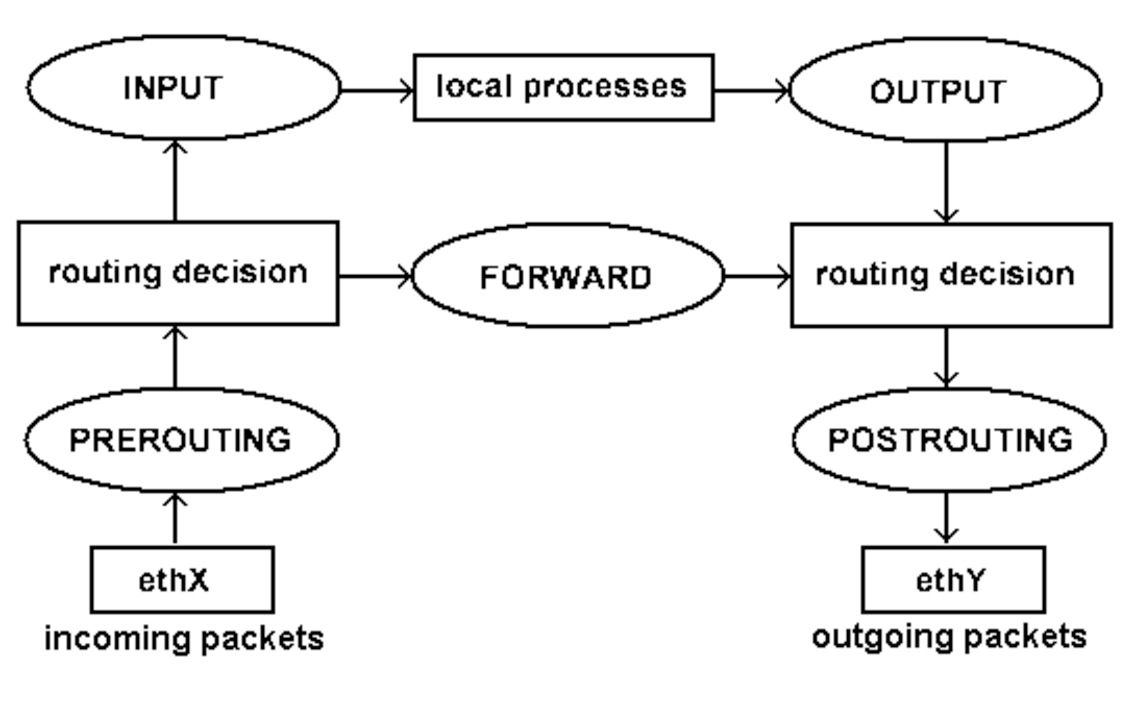
\includegraphics[scale=0.25]{figures/netfilter.pdf} 
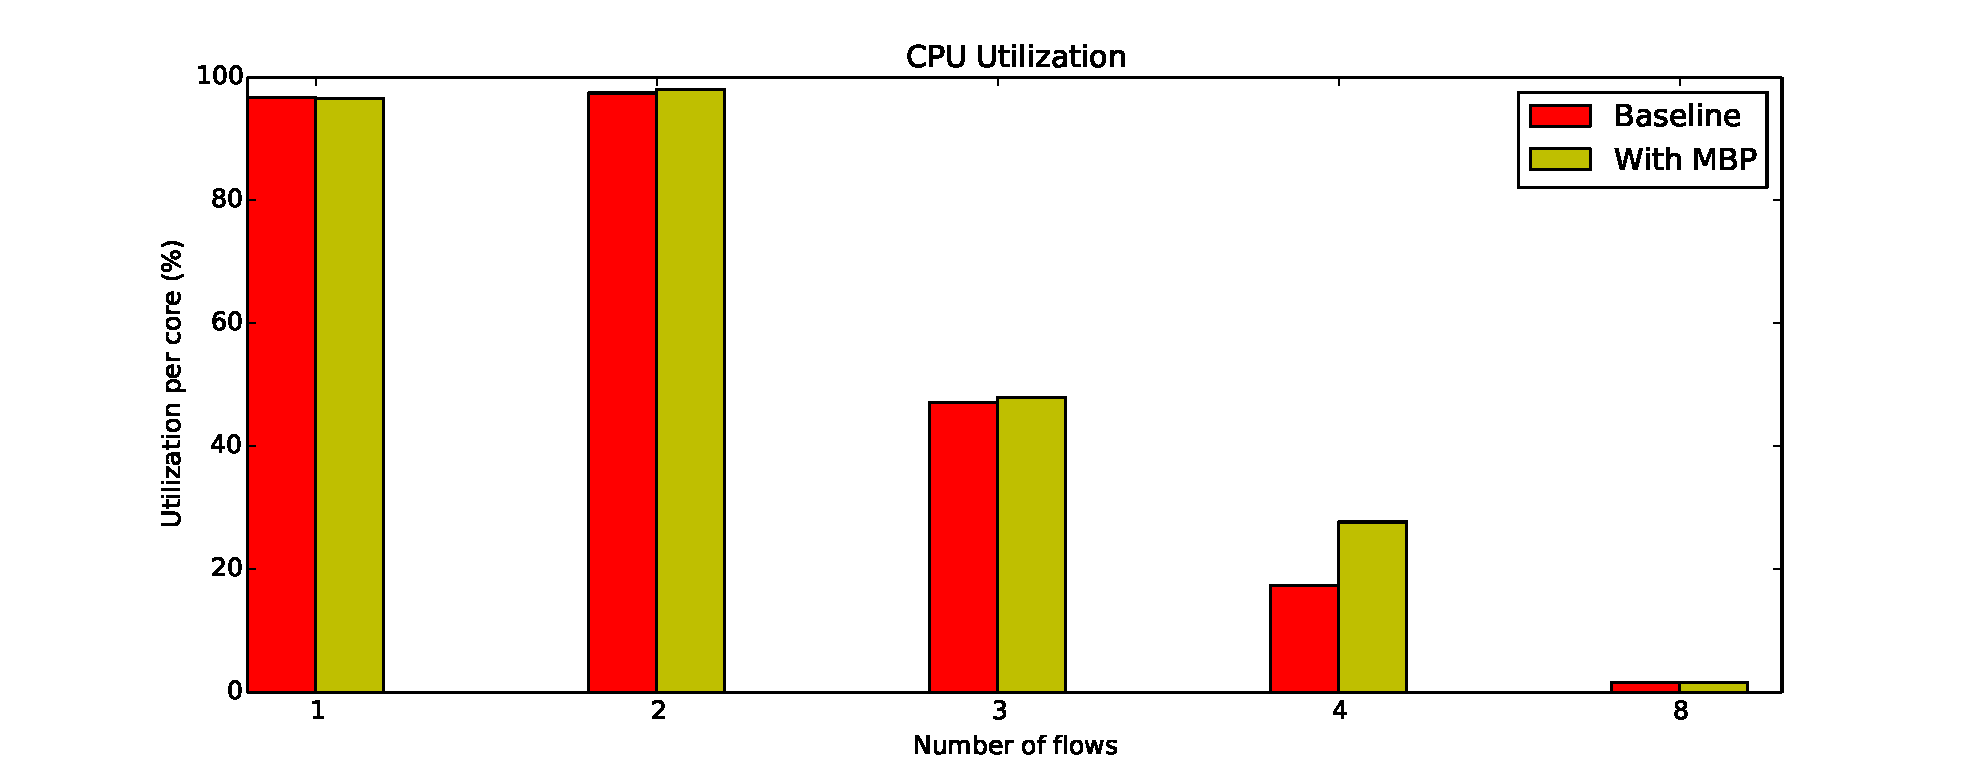
\includegraphics[width=\linewidth]{figures/CPU.pdf} 
% 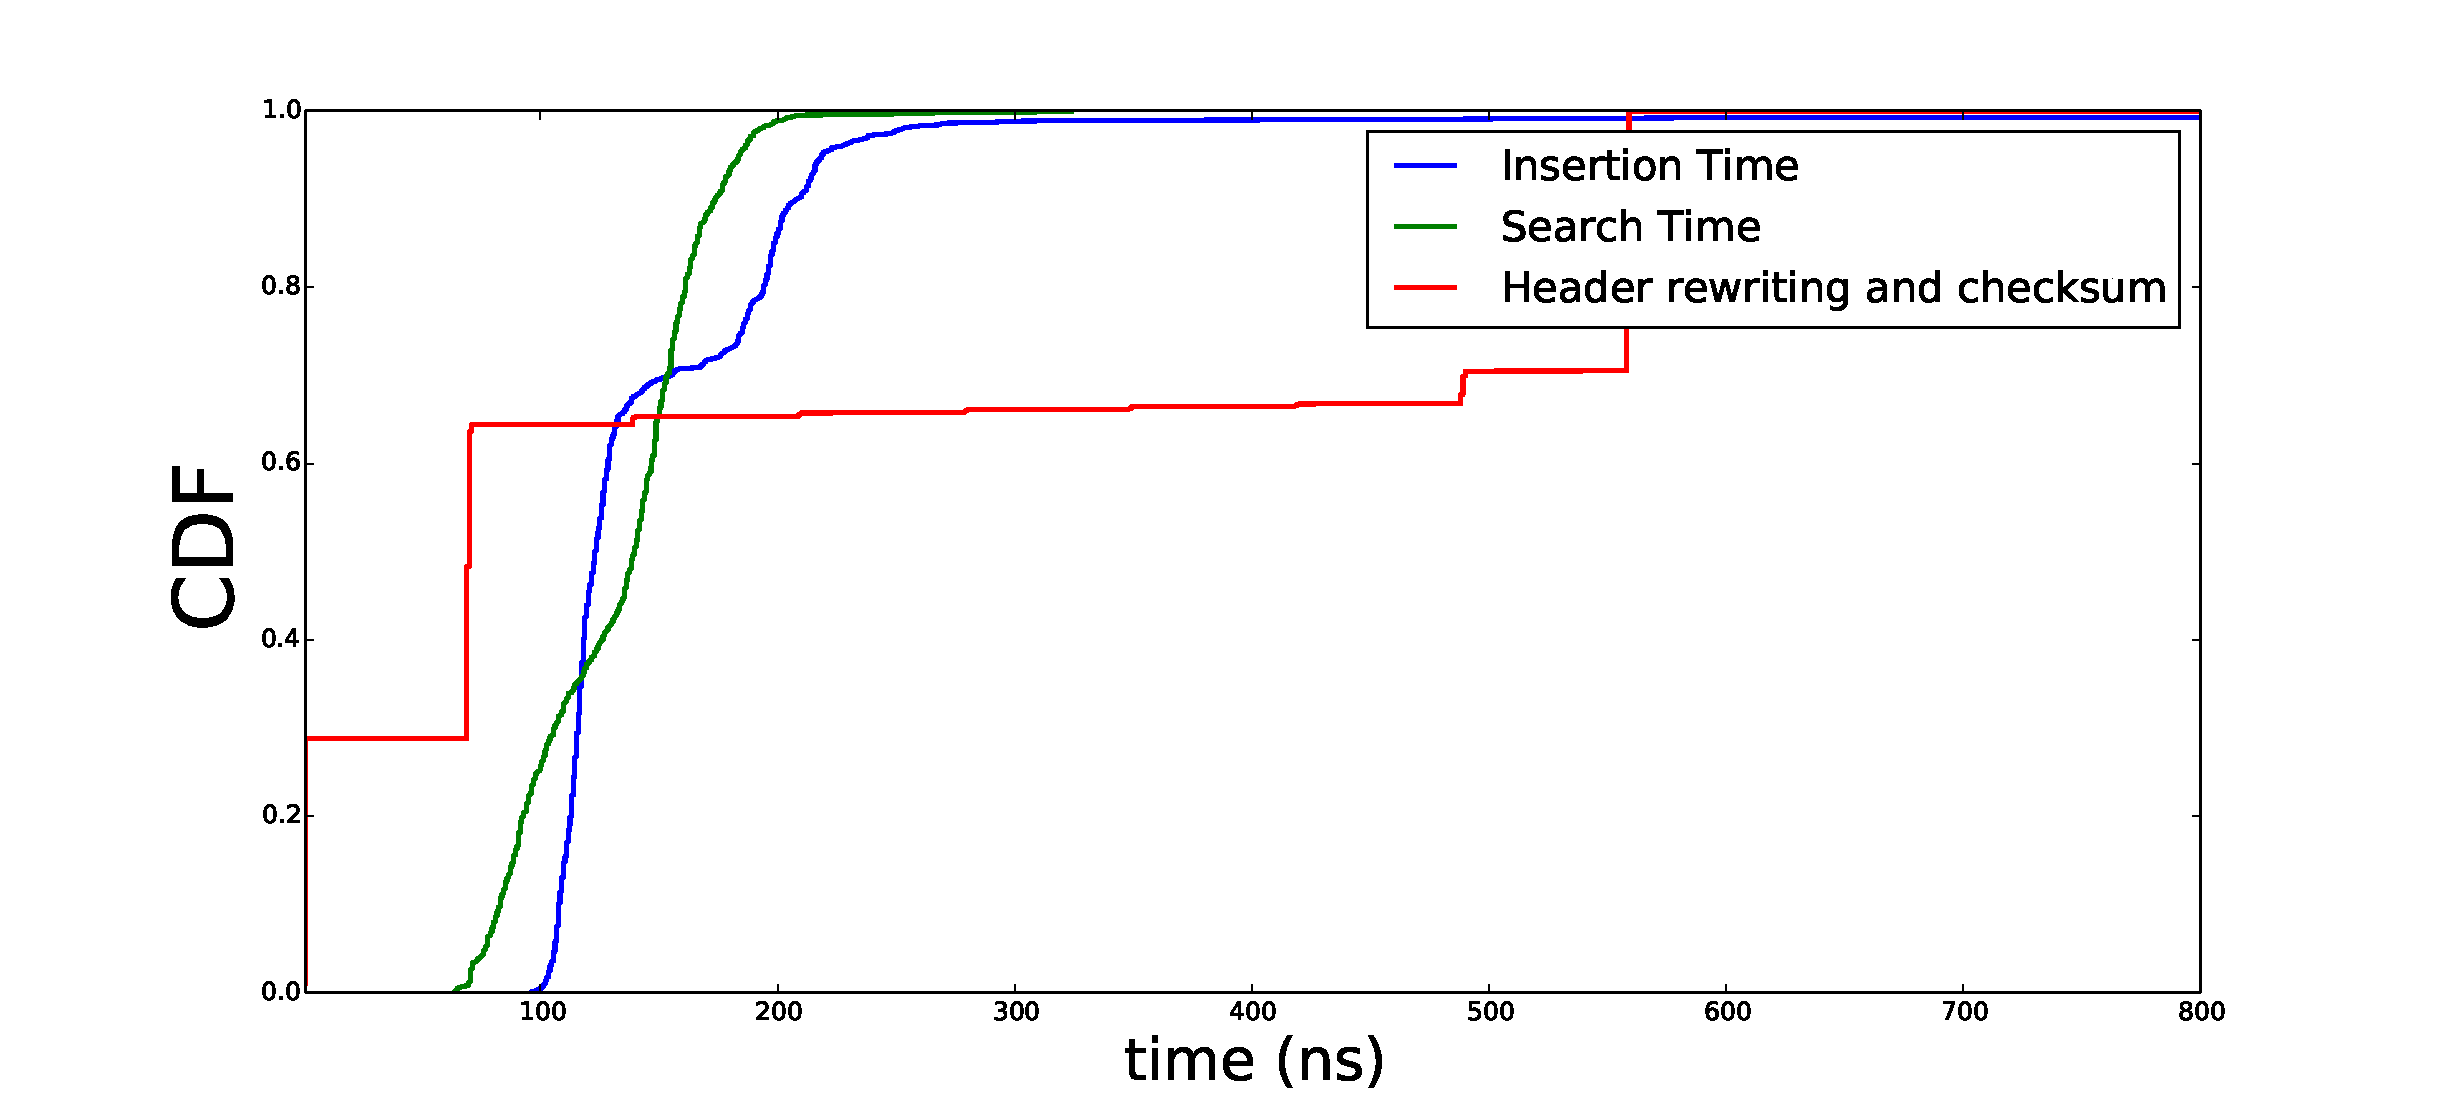
\includegraphics[width=\linewidth]{figures/cdf.pdf} 
\caption{\small Average CPU utilization in stress test. Note we only include the cores that are interrupted by the NIC.}\label{throughput}
\end{figure}

We plotted the CPU utilization of the middlebox in the same experiments. Note since the middlebox acts as a software router without the kernel module, it also consumes a certain amount of CPU cycles. The highest difference between the baseline and the system lies in the setting of 4 flows, the utilization is 10\% higher than that of the vanilla system (27.6\% versus 17.2\%), but under most circumstances the gap is within 2\%. One thing worth noting is that as the number of flow increases, the CPU utilization per core plummets, our explanation is that since the testbed machine has 16 cores and 32 hyper-threads, it spreads out quite evenly, and the CPU utilization scales linearly at high load but it is not the case at low load (e.g., 1M packets/s causes much higher CPU utilization than 500K packets/s). 


The experimental result is promising and proves that the in-kernel data plane implementation can offer very high throughput at the cost of modest increase of CPU utilization. 



\subsection{Latency}
We evaluate our system's latency in the following order: (i) how much overhead it has for a super-session setup? (ii) how much overhead it has during loss-free, packet order-preserving, and substream separation and order preserving update, even in the case of data packet loss or reordering. 


\subsubsection{Three-Way handshake}
% \kelvin{will add more stuff, like three hops, 4 hops and 5 hops, but do get the idea of how to do it now, three hops values are 426.5 28.7515216989, 464.5 22.8527897641, 688.1 24.6473122267}
We first measure the latency for session establishment, in a topology of three hops (client - middlebox - server). We have two different implementation, (i) out of band UDP ahead to TCP handshake, (ii) piggyback TCP handshake at the payload. Not surprisingly, TCP piggyback can greatly reduce the extra latency due to propagation delay, with a modest increase less than $40 \mu $s. On the other hand, out-of-band UDP incurs $688\mu$s delay ahead of TCP handshake. 

\begin{figure}[ht]
\centering
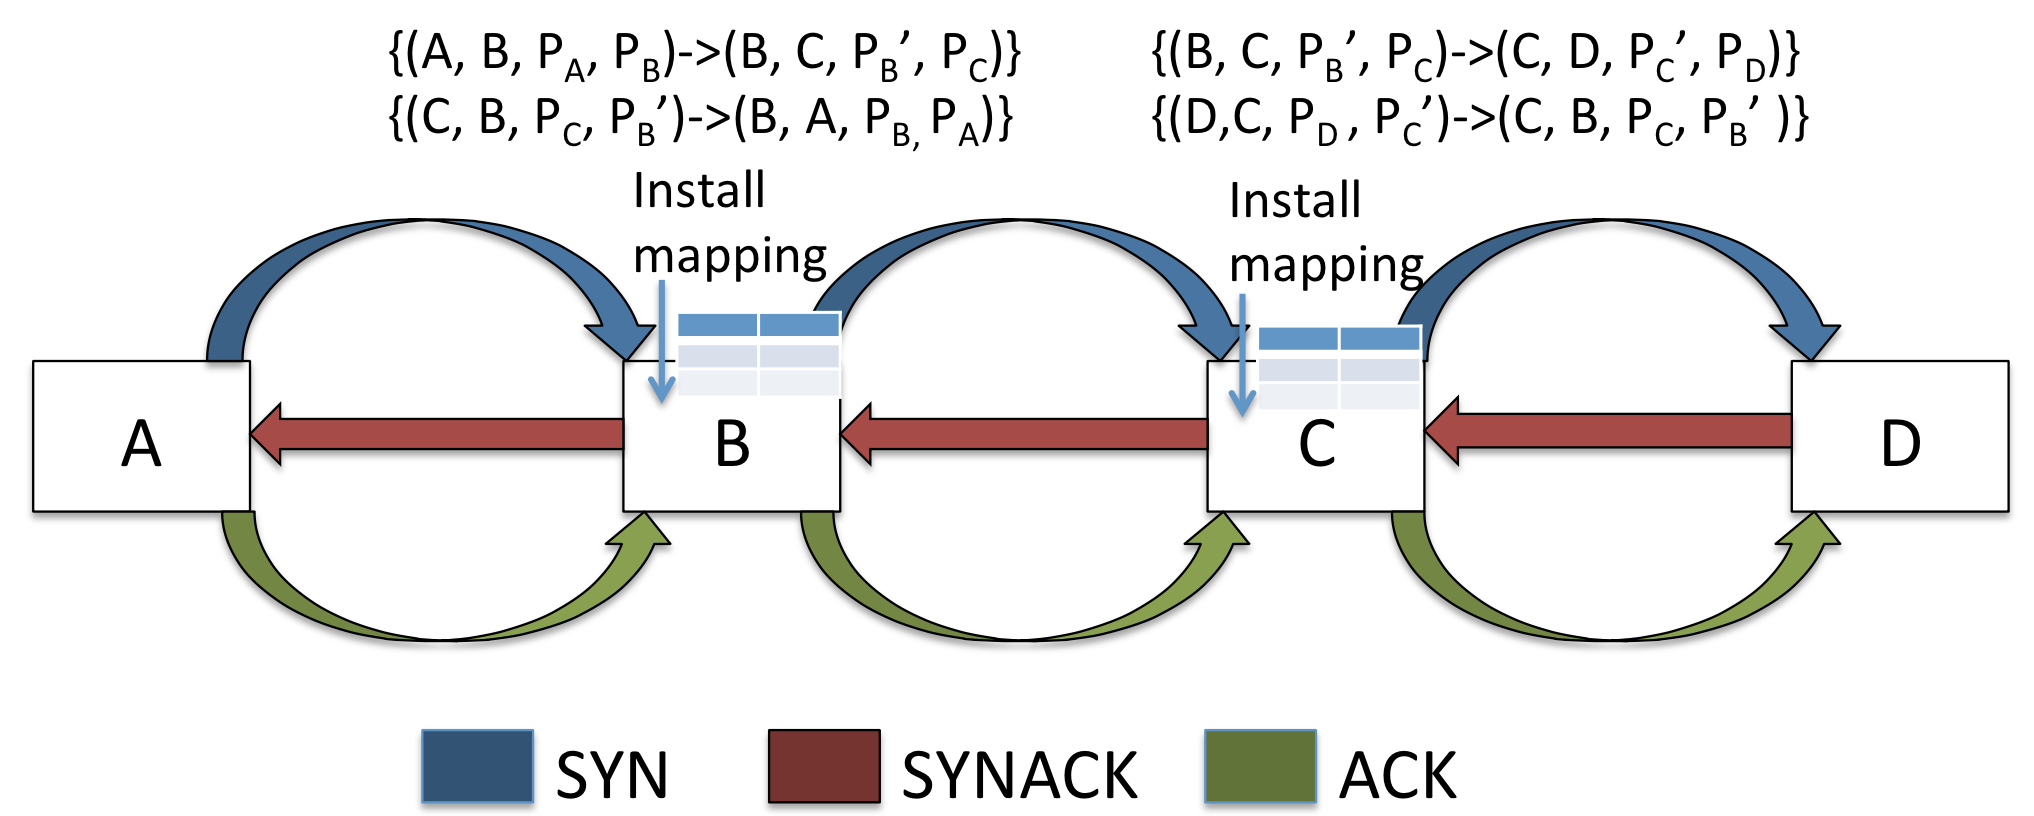
\includegraphics[width=\linewidth]{figures/threeway.png} 
\caption{\small Latency for session establishment}\label{threeway}
\end{figure}
\subsubsection{Flow Migration}
\system supports flow migrations with various properties. We also measure the time interval for a loss-free, order-preserving, and byte stream order preserving update.   

We run our experiments in a topology with four middleboxes (A,B,C,D), there are two paths (A-B-D) and (A-C-D) that each consists of three middleboxes. The goal of the flow migration is to replace middlebox B with D. We measure the latency for such migration, using (a) loss-free migration, (b) order-preserving migration, and (c) (a different property). The latency are evaluated under different loads on a network with all 1Gbps links. 

As shown in the table, we can see that not surprisingly, as the load of the network increases, the update latency increases. We attribute the increase to two causes, the queuing delay in the network and the scheduling delay in local servers. In loss-free migration, the old path is saturated; however, the new path is idle and thus the increase is due to the high load in server. In order-preserving migration, the update is on hold until both the new and old paths have sent notification, and thus the queuing delay also contributes to the latency. 

\begin{table}[ht]
\centering
\small
\begin{tabular} {|c |c | c| c|}

\hline
Load&Loss-Free& Order-Preserving\\ \hline 

\textbf{0\% }  &1.7ms & 2.3ms \\ \hline
\textbf{50\% }  & 2.1ms &2.6ms \\ \hline
\textbf{100\% }  & 3.6ms &14ms \\ \hline

\end{tabular}
\caption{Flow migration update time under different network load} \label{movelatency} 
\end{table}

The results demonstrate that the system can deal with flow migrations in the order of tens of milliseconds. To put in perspective, the time for a middlebox state migration is above 100ms~\cite{splitmerge, OpenNF} and a fast consistent update takes up to a second~\cite{xinjin}, a more detailed breakdown is in table~\ref{latencycomp}.

\begin{table}[ht]
\centering
\small
\begin{tabular} {|c |c | c| c|}

\hline
 &Loss-Free& Order-Preserving \\ \hline 
% &~\cite{SIMPLE,FLOWTAGS, OpenNF}& ~\cite{CoMB, splitmerge}& ~\cite{ Aplomb,DOA,I3} & ~\cite{OVS, Netfilter} & \\ \hline

Split/Merge
\footnote{\scriptsize at packet rate 37.5 kpps, time are consumed across flow migration and state migration} 
		&~500ms&$\otimes$\footnote{\small not supported} \\ \hline
OpenNF(a)
\footnote{\scriptsize flow update time at packet rate 2.5-10 kpps, (a) is for flow migration time, and (b) is for middlebox state migration time} 
	       & 84ms& 96ms\\ \hline
OpenNF(b)      & 134ms& 208ms \\ \hline
Dionysus
\footnote{\scriptsize Large scale networks}
	      &600-1200ms &$\otimes$  \\ \hline
Our system
\footnote{\scriptsize at packet rate 75 kpps (900 Mbps)} 
	    & 4ms &14ms \\ \hline

\end{tabular}
\caption{Comparison with other dynamic middlebox and flow migration systems}\label{latencycomp} 
\end{table}

